\documentclass{article}
\usepackage[utf8]{inputenc}
\usepackage{amsmath, amssymb}
\usepackage{mathtools}
\usepackage{a4wide}
\usepackage{appendix}
\usepackage{listings}
\usepackage{float}
\usepackage{subcaption}


\title{Optic flow}
\author{Hugo (s214734) \and Mikael H. Hoffmann (s214753) \and (s211469) \and Jacob Tuxen (s194572)}
\date{\today}

\begin{document}

\maketitle

\section{Introduction (problem and background) - Hugo}
Optical flow is a method to determine object motion in video, based on the relative displacement of pixels
through time in the video. To obtain such a motion prediction, a few strong assumptions are made
about the subject video, including:
\begin{itemize}
    \item There has been only a small displacement through time
    \item There are no changes in the lighting
    \item Pixel intensity alone is enough to determine movement in the video
\end{itemize}
These assumptions are necessary for applying a mathematical model to the problem of optic flow.

\section{Data and experiments}




\section{Mathematical model and image processing methodology}
We start by considering the point $\boldsymbol{p} = [p_x, p_y, p_t]$ and we want to find vector $\boldsymbol{u} = [x, y, 1]$ which represents the movement of the above mentioned pixel in \emph{one} time frame, which is given by

\begin{equation}\label{eq:initial-equation}
    \boldsymbol{V(p + u)} - \boldsymbol{V(p)} = 0.
\end{equation}

Here $\boldsymbol{V}$ represents the pixel value at $\boldsymbol{p}$ - therefore the above is equivalent to brightness constancy constraint. 

If the displacement is small then it is possible to  approximate the movement with a first order Taylor expansion

\begin{equation}
    \boldsymbol{V(p + u)} = \boldsymbol{V(p)} + \begin{bmatrix}
        \boldsymbol{V}_x(\boldsymbol{p}) & \boldsymbol{V}_y(\boldsymbol{p}) & \boldsymbol{V}_t(\boldsymbol{p})
    \end{bmatrix} \boldsymbol{u}.
\end{equation}
Where $[\boldsymbol{V}_x(\boldsymbol{p}),\boldsymbol{V}_y(\boldsymbol{p}),\boldsymbol{V}_t(\boldsymbol{p})]$ are the value of the gradient in the $x,y,t$ directions respectively. Inserting this in equation \ref{eq:initial-equation} yields

\begin{equation}
    \begin{split}
        \boldsymbol{V(p)} + \begin{bmatrix}
        \boldsymbol{V}_x(\boldsymbol{p}) & \boldsymbol{V}_y(\boldsymbol{p}) & \boldsymbol{V}_t(\boldsymbol{p})
        \end{bmatrix} \boldsymbol{u} - \boldsymbol{V(p)} &= \boldsymbol{V}_x(\boldsymbol{p}) x + \boldsymbol{V}_y(\boldsymbol{p}) y + \boldsymbol{V}_t(\boldsymbol{p}) \cdot 1 \\
        &= 0,
    \end{split}
\end{equation}

and rearranging gives

\begin{equation}\label{eq:final-model}
    \boldsymbol{V}_x(\boldsymbol{p}) x + \boldsymbol{V}_y(\boldsymbol{p}) y = -\boldsymbol{V}_t(\boldsymbol{p}).
\end{equation}

\subsection{Lucas Kanade solution}
The equation in (\ref{eq:final-model}) is an under determined since there is one equation with 2 unknowns, it is not possible to determine a solution for $x$ and $y$. Considering a point $\textbf{p}=[p_x,p_y,p_t]$, Lucas Kanade's method suggest to assume that all pixels within a small neighborhood of $\textbf{p}$ have the same movement. This assumptions implies that (\ref{eq:final-model}) can be expanded by solving for all points within the neighborhood of \textbf{p}, which yields the following system.
\begin{equation}\label{LK}
    \begin{bmatrix}
        \vdots & \vdots \\
        \boldsymbol{V}_x(\boldsymbol{p}_i) & \boldsymbol{V}_y(\boldsymbol{p}_i) \\
        \vdots & \vdots
    \end{bmatrix} \begin{bmatrix}
        x \\ y
    \end{bmatrix}
    = - \begin{bmatrix}
        \vdots \\ \boldsymbol{V}_t(\boldsymbol{p}_i) \\ \vdots
    \end{bmatrix}.
\end{equation}
The system in (\ref{LK}) is an over determined linear system with $n$ equations and 2 unknowns, where $n$ is the number of pixels in the neighbourhood around \textbf{p}. Such a system can be solved using least squares.

To conclude the optical flow in each pixel is obtained by assuming that each pixels within a small neighbourhood of each share the same movement. 

\subsection{Image processing methodology}
In image processing an image is expressed as a single matrix for gray scale images and 3 matrices for RGB images. This representation allows us to manipulate the images using linear algebra and other areas of mathematics involving matrices. In the given problem for optical flows the calculations rely on image gradients, Taylor expansions and linear least squares. 

\section{Visualise results - Mikael}
When running the code with the supplied test video and our custom video we got the following

\begin{figure}[H]
    \begin{subfigure}{.5\textwidth}
        \centering
        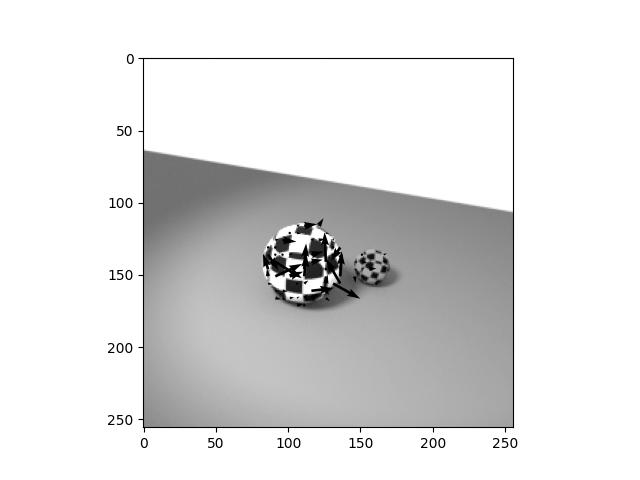
\includegraphics[scale=0.4]{code/toyProblem_F22_vectorField/48.jpg}
        \caption{The 48th frame with arrows indicating the size and movement of selected pixels.}
        \label{fig:moving-ball}
    \end{subfigure}%
    \begin{subfigure}{.5\textwidth}
        \centering
        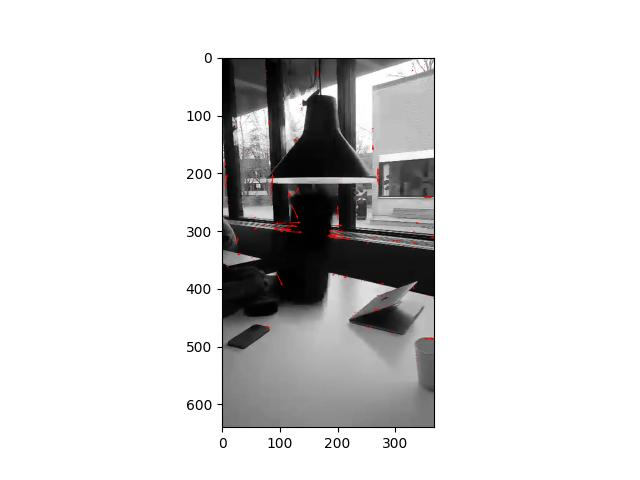
\includegraphics[scale=0.4]{code/vanteImages_vectorField/32.jpg}
        \caption{Placeholder!}
        \label{fig:custom-video}
    \end{subfigure}
\end{figure}

In both cases we see that 

\section{Discuss results - }

\section{Conclude - Hugo}
A complete python implementation of the Lucas Kanade solution and some of its variations, to the optical flow problem, is created and applied to various optical flow problems. These are used to illustrate both strengths and weeknesses of the Lucas Kanade optical flow solution - see figures ???, ??? and ???.
% By applying the Lucas Kanade method to optical flow, we have shown the dependency of optical flow to lighting conditions. Moreover 





\section{Exercise (5)}
Define $A$ as per equation (2) in the handout:
\begin{equation}
    A = \begin{bmatrix}
    \vdots & \vdots \\
    V_{x}(p_i) & V_{y}(p_i) \\
    \vdots & \vdots
    \end{bmatrix}
\end{equation}
Then the normal equation to $Ax = b$ will have the system matrix (where $N$ denotes the considered neighborhood):
\begin{equation}
    A^\intercal A = \begin{bmatrix}
        \sum_{i \in N} V_{x}(p_i)^{2} & \sum_{i \in N} V_{x}(p_i)V_{y}(p_i) \\
        \sum_{i \in N} V_{x}(p_i)V_{y}(p_i) & \sum_{i \in N} V_{y}(p_i)^{2}
    \end{bmatrix}
\end{equation}
Which we could also get by passing a filter of all ones over $N$ in $V_x$ and $V_y$.

\newpage
\appendix
\section{Code}
\subsection{Exercise 1}
\lstinputlisting[language=Python,breaklines=true]{code/exercise_1.py}

\subsection{Exercise 2}
\lstinputlisting[language=Python,breaklines=true]{code/exercise_2.py}

\subsection{Exercise 3}
\lstinputlisting[language=Python,breaklines=true]{code/exercise_3.py}

\subsection{Various functions}
\lstinputlisting[language=Python,breaklines=true]{code/functions.py}

\subsection{Video plotter}
\lstinputlisting[language=Python,breaklines=true]{code/video_plotter.py}

\subsection{Main}
\lstinputlisting[language=Python,breaklines=true]{code/main.py}


\end{document}
